\documentclass{beamer}

\usepackage[textsize=footnotesize]{todonotes}

\usetheme[compress]{Singapore}
\setbeamertemplate{footline}[frame number]
\setbeamercovered{transparent}
\beamertemplatenavigationsymbolsempty
%\setbeamertemplate{navigation symbols}{}

\title{\uppercase{Electric Vehicle X Driving Range Prediction - EV X DRP}}
\subtitle{Relatório de progresso}
%\subtitle{}
\author{
	{\large David P. Coutinho \qquad Artur J. Ferreira} \\
	{\qquad \hspace{-1cm} david.coutinho@isel.pt \qquad arturj@isel.pt} \\
    {\vspace{1cm}}
    {\large David A. S. G. Albuquerque} \\
    {A43566@alunos.isel.pt}
}
\institute
{
	\vspace{0.5cm} \\
	{\normalsize Instituto Superior de Engenharia de Lisboa } \\
}
\date{
	\vspace{-0.75cm}
	Friday, 25 March 2022
}

\usepackage[style=alphabetic]{biblatex}
\addbibresource{bibliography.bib}

\begin{document}

\begin{frame}[t,plain]
    \titlepage
\end{frame}

\begin{frame}
    \frametitle{Outline}
    \tableofcontents
\end{frame}

\section[Introdução]{Introdução}
\subsection[Objetivo]{Objetivo}
\begin{frame}
\frametitle{Introdução - Objetivo}

\begin{itemize}
	\item Realizar estimativas da distância de condução restante 
	que um veículo elétrico pode efetuar relativamente à sua autonomia - \textit{eRange};
\end{itemize}

\begin{figure}[H]
    \begin{center}
        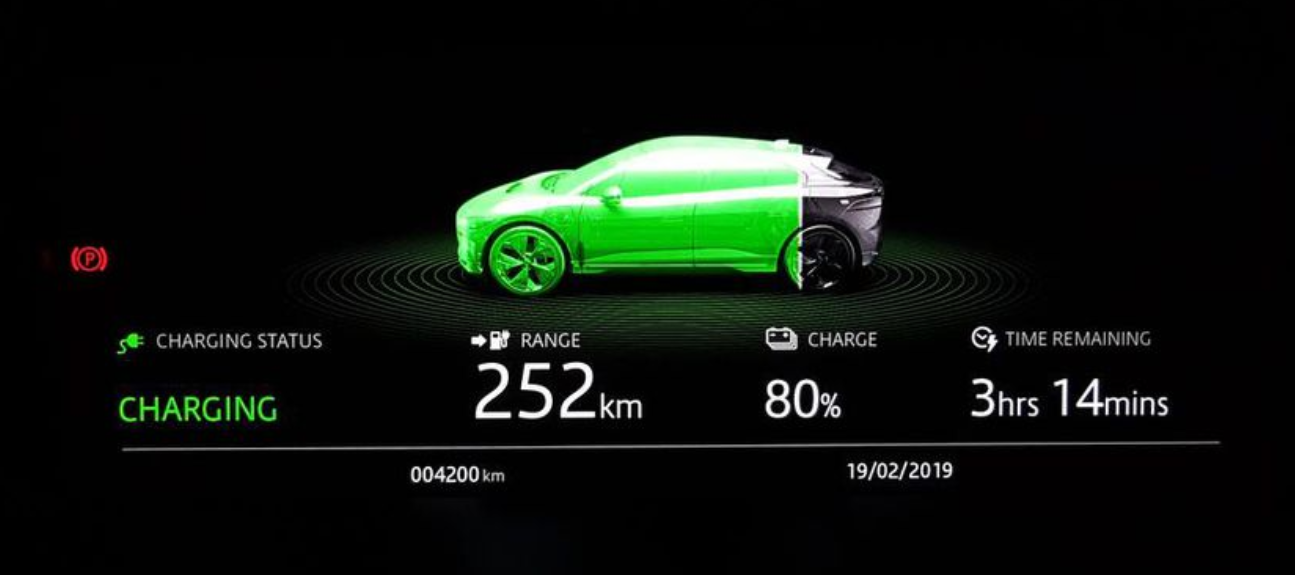
\includegraphics[scale=0.25]{./figures/erange_gauge}
    \end{center}
\end{figure}

\end{frame}


\subsection[eRange]{O que é eRange?}
\begin{frame}
\frametitle{Introdução - O que é eRange?}

\begin{itemize}
	\item A distância máxima que um veículo elétrico consegue viajar;
	\item Alivia a ansiedade do condutor; 
	\item Depende de vários dados da condução do veículo:
		  \begin{itemize}
			  \item SOC (State of charge) - indica o estado de carga da bateria;
			  \item Estado do ar condicionado;
			  \item Travagem regenerativa;
			  \item Inclinação da estrada;
			  \item (entre outros)
		  \end{itemize}
\end{itemize}


\end{frame}

\subsection[Problema]{O problema de estimação}
\begin{frame}
\frametitle{Introdução - O problema}

\begin{itemize}
	\item Dependência de vários fatores;
	\item Escassez de \textit{datasets};
	\item Escolha dos algoritmos de \textit{machine learning};
\end{itemize}

\end{frame}

\subsection[Como resolver]{Como resolver}
\begin{frame}
\frametitle{Introdução - Como resolver}

\begin{itemize}
	\item Uso de inteligência artificial para a resolução do problema;
	\item Aprendizagem através de \textit{datasets} de viajens de carros electricos;
\end{itemize}

\end{frame}

\section[Estado da arte]{Estado da arte}
\subsection[Datasets]{Datasets}
\begin{frame}
\frametitle{Estado da arte - \textit{Datasets}}

\begin{itemize}
	\item \textit{EV Database} (ev-database.org) \footfullcite{onlineEvDatabase};
	\item \textit{VED Dataset} \footfullcite{vedDatasetCleared};
		  \begin{itemize}
			  \item Dados reais de condução de veículos elétricos (2013 Nissan leaf)  
		  \end{itemize}
	\item \textit{Emobpy} \footfullcite{emobpyCleared}.
		  \begin{itemize}
			  \item Geração de dados de condução de veículos elétricos.
		  \end{itemize}
\end{itemize}

\end{frame}

\subsection[\textit{Datasets} de condução]{Datasets}
\begin{frame}
\frametitle{Estado da arte - \textit{Datasets} de condução}


\end{frame}

\subsection[Implementacoes]{Implementações}
\begin{frame}[label={Implementacoes}]
\frametitle{Estado da arte - Implementações}

\let\oldfootnotesize\footnotesize
\renewcommand*{\footnotesize}{\oldfootnotesize\tiny}

\begin{itemize}
	\item Uso combinado de \textit{Gradient Boosting Regression Trees}
		  \footfullcite{machineLearningERangeGradientBoostRtsCleared};
	\item \textit{Ensemble learning} \footfullcite{eRangeMachineLearningEnsembleCleared} com: 
		  \begin{itemize}
			  \item \textit{Decision Tree };
			  \item \textit{Random Forest};
			  \item \textit{K-Nearest Neighbor}.
		  \end{itemize}
	\item \textit{Self-Organizing Maps}\footfullcite{eRangeMachineLearningGHSOMCleared} 
		  (e híbridos com \textit{Regression Trees} \footfullcite{machineLearningERangeSOMandRtsCleared});
	\item Redes neuronais com \textit{Multiple Linear Regression} 
		  \footfullcite{eRangeMachineLearningNeuralnetworkMLRCleared}.
\end{itemize}

\renewcommand*{\footnotesize}{\oldfootnotesize}

\end{frame}

\section[Trabalho realizado]{Trabalho realizado}
\begin{frame}
\frametitle{Trabalho realizado}

\begin{itemize}
	\item Estudo do problema e soluções existentes;
	\item Escolha de um \textit{dataset} válido;
	\item Implementação de um modelo de baseado em historial \footfullcite{classicEVXCleared2}.
\end{itemize}

\end{frame}

\section[Trabalho futuro]{Trabalho futuro}
\subsection{Objetivos futuros}
\begin{frame}
\frametitle{Trabalho futuro}

\begin{itemize}
	\item Arquitetura de projeto:
		  \begin{itemize}
			  \item Escolha do algoritmo de \textit{machine learning};
		  \end{itemize} 
	\item Implementação do projeto:
		  \begin{itemize}
		      \item Integração do \textit{dataset};
		      \item Implementação do modelo;
		  \end{itemize}
	\item Testes;
	\item Recolha de resultados.
\end{itemize}

\end{frame}

\subsection{Diagrama}
\begin{frame}
\frametitle{Trabalho futuro - Diagrama}

\begin{center}
	\begin{figure}[H]
		\begin{center}
			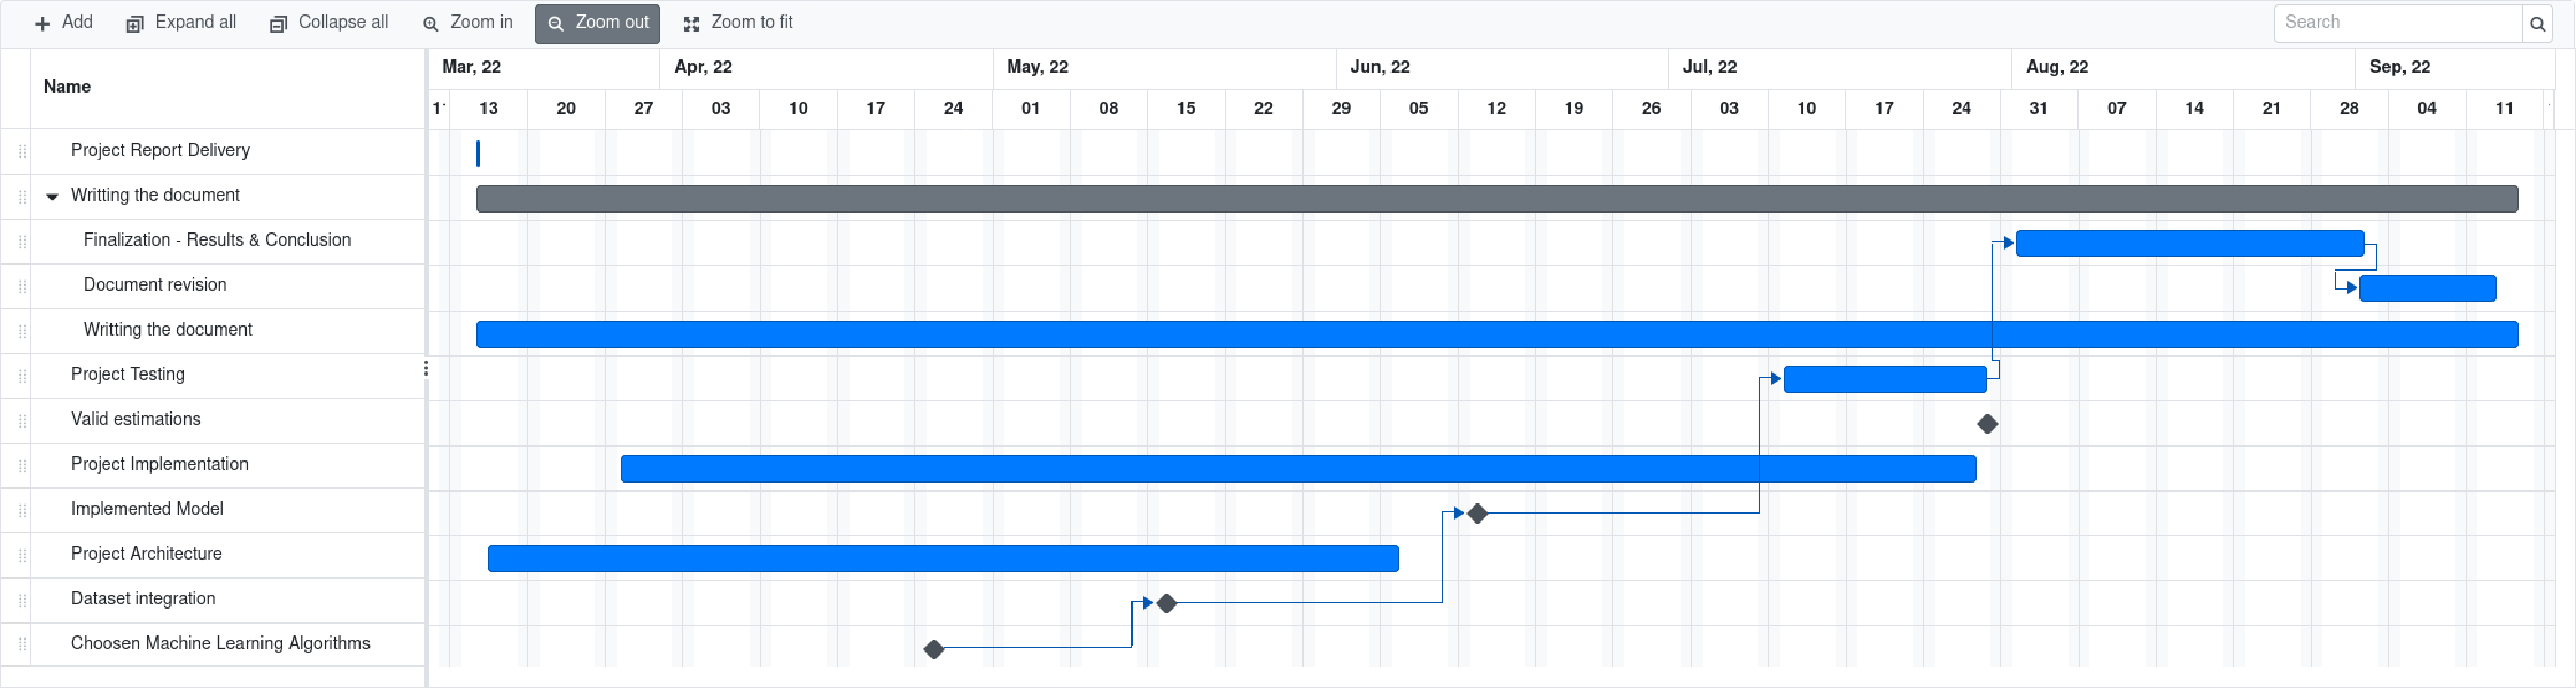
\includegraphics[scale=0.16]{./figures/planning_tiny1.pdf}
		\end{center}
	\end{figure}
\end{center}


\begin{figure}[H]
    \begin{center}
        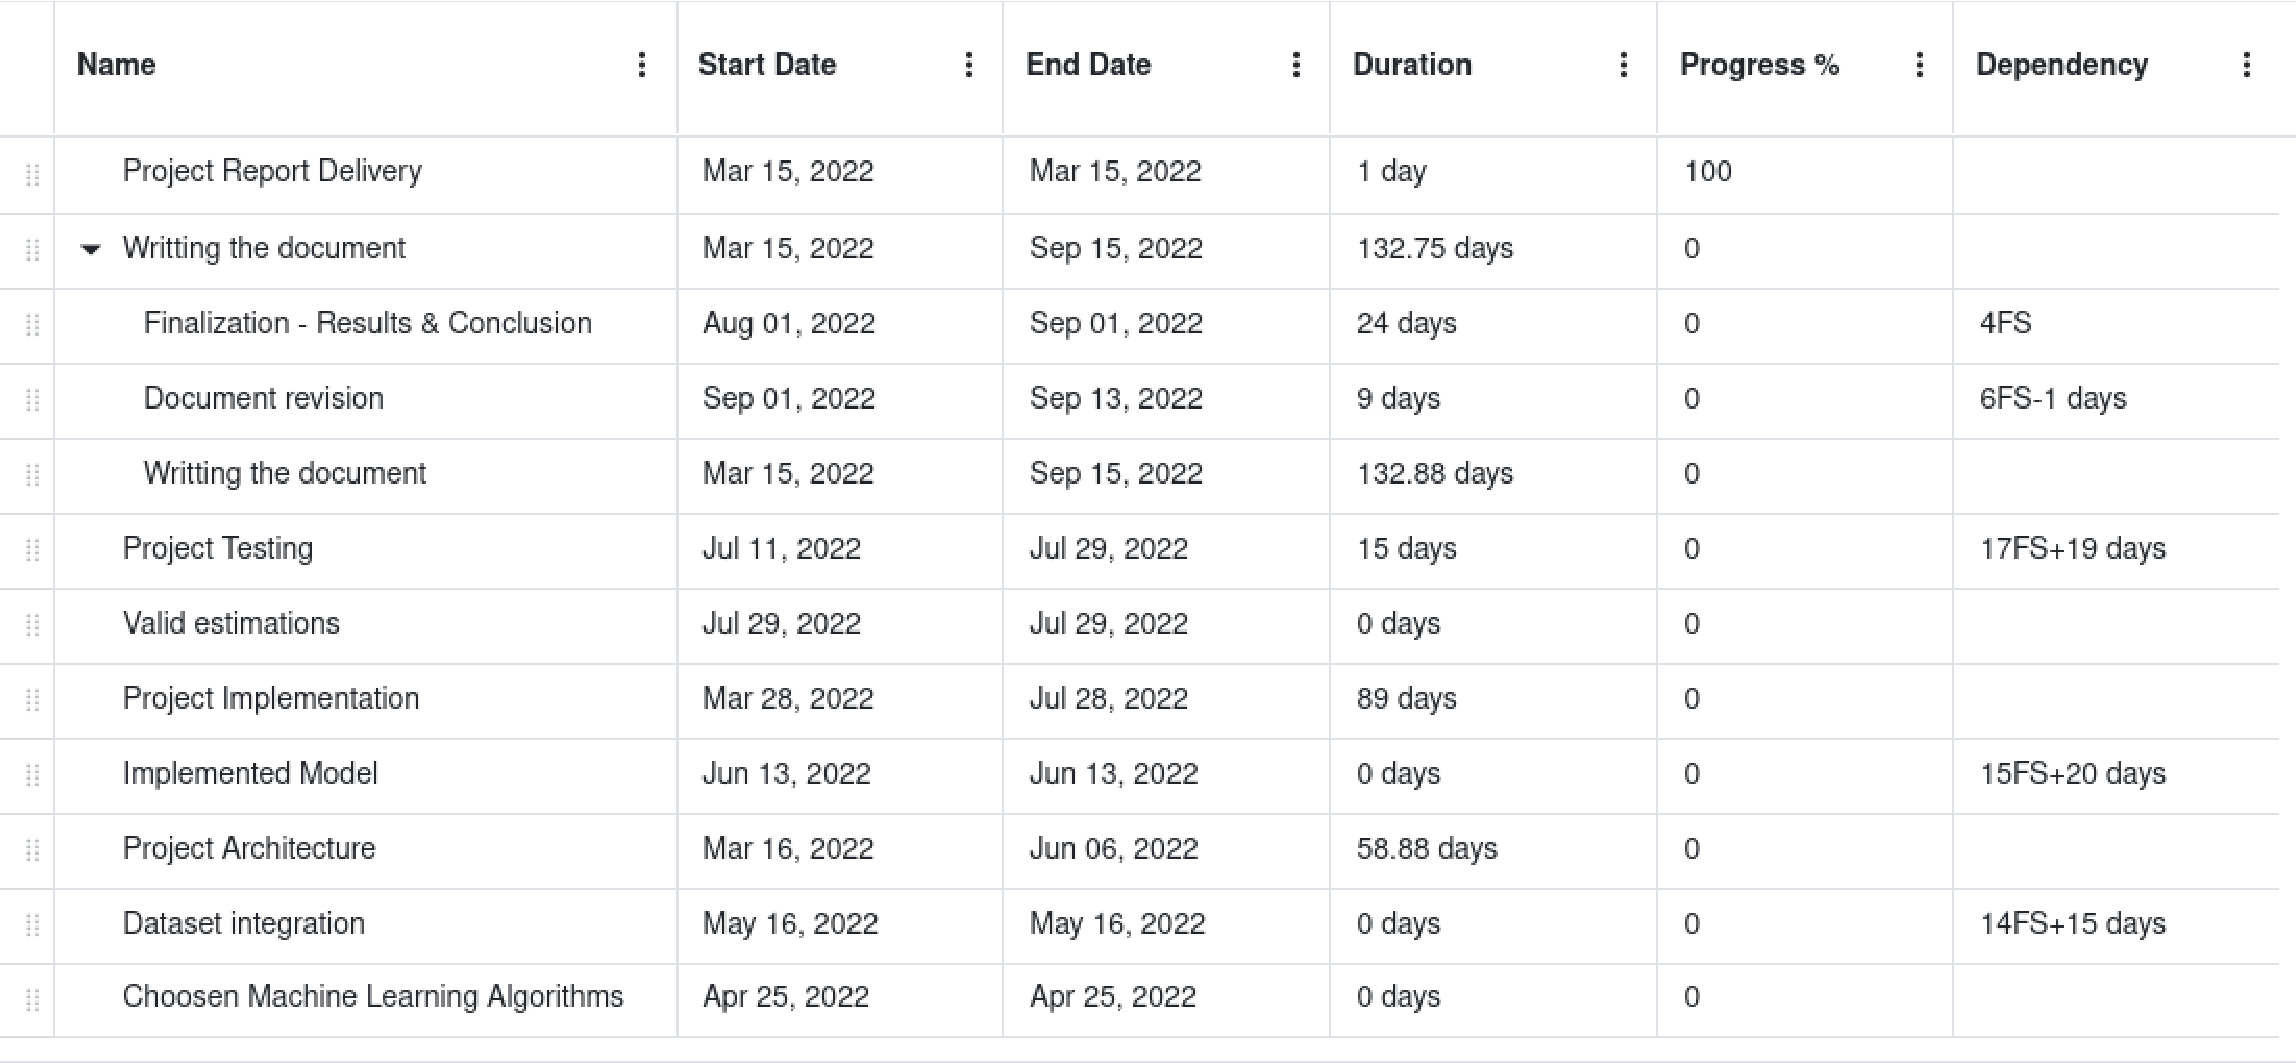
\includegraphics[scale=0.20]{./figures/planning_tiny2.pdf}
    \end{center}
\end{figure}

\end{frame}

\end{document}